\documentclass[11pt]{article}

% Change "review" to "final" to generate the final (sometimes called camera-ready) version.
% Change to "preprint" to generate a non-anonymous version with page numbers.
\usepackage[final]{acl}

% Standard package includes
\usepackage{times}
\usepackage{latexsym}

% For proper rendering and hyphenation of words containing Latin characters (including in bib files)
\usepackage[T1]{fontenc}
% For Vietnamese characters
% \usepackage[T5]{fontenc}
% See https://www.latex-project.org/help/documentation/encguide.pdf for other character sets

% This assumes your files are encoded as UTF8
\usepackage[utf8]{inputenc}

% This is not strictly necessary, and may be commented out,
% but it will improve the layout of the manuscript,
% and will typically save some space.
\usepackage{microtype}

% This is also not strictly necessary, and may be commented out.
% However, it will improve the aesthetics of text in
% the typewriter font.
\usepackage{inconsolata}

%Including images in your LaTeX document requires adding
%additional package(s)
\usepackage{graphicx}

% Additional packages
\usepackage{booktabs}
\usepackage{pgfplots}
\pgfplotsset{compat=1.18}
\usepackage{listings}
\usepackage{xcolor}
\usepackage{multirow}
\usepackage{enumitem}
\usepackage{float}
\usepackage[most]{tcolorbox}
\usepackage{pifont}

% If the title and author information does not fit in the area allocated, uncomment the following
%
%\setlength\titlebox{<dim>}
%
% and set <dim> to something 5cm or larger.

% YAML listings style for prompt templates
\lstdefinestyle{yaml}{
  basicstyle=\tiny\ttfamily,
  breaklines=true,
  frame=single,
  backgroundcolor=\color{gray!5},
  rulecolor=\color{gray!40},
  xleftmargin=2pt,
  xrightmargin=2pt,
  aboveskip=4pt,
  belowskip=4pt,
  columns=fullflexible,
  keepspaces=true,
  showstringspaces=false,
}

\title{Rasende Rakete at SemEval-2026 Task 6: LLM-First Approach with Iterative Prompt Repair for Classifying Evasion in Political Interviews}

\author{
 \textbf{Omar Elbeltagui\thanks{Equal contribution}},
 \textbf{Nils Knittel\footnotemark[1]},
 \textbf{Leonie Süß\footnotemark[1]},
 \textbf{Umut Yıldırır\footnotemark[1]},
 \textbf{Qiyan Zhai\footnotemark[1]}
\\
 Technical University of Munich
\\
\\
 \small{
   \texttt{\{omar.elbeltagui, nils.knittel, leonie.suess, umut.yldrr, qiyan.zhai\}@tum.de}
   }
}

\begin{document}
\maketitle
%% ===
%% ABSTRACT
%% ===
\begin{abstract}
%Large language models have been shown to achieve state-of-the-art results in various classification tasks.
We describe our system for SemEval-2026 Task 6 (CLARITY), which addresses automatic detection of evasive responses in political interviews.
%Given a political question-answer pair, the system classifies the response's clarity level and identifies specific evasion techniques.
We adopt an LLM-first approach built around two core contributions:
(i)~an \emph{iterative prompt repair loop} that diagnoses classification errors on concrete failure examples and applies prompt revisions, improving F1 for evasion techniques by +13.7pp over the base prompt; and
(ii)~a \emph{configurable end-to-end Java Pipeline} that supports multiple LLM providers, strategies, and systematic experimentation.
Our best system achieves 0.831 accuracy and 0.797 F1 on clarity level classification (Sub-task 1) and 0.620 accuracy and 0.575 F1 on evasion technique classification (Sub-task 2), improving over \citet{thomas2024isaidthatdataset} by +11.8pp accuracy and +11.5pp F1.
\end{abstract}

%% ===
%% 1 INTRODUCTION
%% ===
\section{Introduction}

Politicians systematically evade questions in interviews, undermining transparency and accountability.
Detecting such evasion automatically is difficult: evasive behavior is often subtle, context-dependent, and spans a spectrum from vague replies to outright refusals.
SemEval-2026 Task 6, CLARITY \citep{thomas2024isaidthatdataset}, addresses this problem as two sub-tasks on English-language political interview question-answer (QA) pairs of US-Presidents.
Sub-task~1 (Clarity Category) requires classifying responses into three categories: \emph{Clear Reply}, \emph{Ambivalent}, or \emph{Clear Non-Reply}.
Sub-task~2 (Evasion Technique) demands fine-grained identification of 9 evasion techniques (e.g., \emph{Dodging}, \emph{Deflection}, \emph{Declining to answer}; see Figure~\ref{fig:taxonomy}).
Systems must reason about the relationship between intent of the question and content of the answer within real-world political discourse, making this a challenging task at the intersection of discourse analysis and natural language understanding.
We present an LLM-first pipeline with a configuration-based design that enables systematic exploration of models, strategies, and prompt variants.
Following the hierarchical evasion taxonomy of \citet{thomas2024isaidthatdataset}, we classify at the fine-grained 9-category level and map back to the coarse clarity labels, which consistently improves clarity prediction.
Our contributions are:
\begin{enumerate}[nosep,leftmargin=*]
    \item An end-to-end configurable Java pipeline for reproducible LLM-based classification with multi-provider support.
    \item An iterative prompt repair loop: LLM-driven error diagnosis on concrete failure examples followed by surgical prompt revision (\S\ref{sec:prompt-repair}).
    \item Systematic evaluation over 10+ models, different classification strategies and preprocessing options.
\end{enumerate}
Our code and configurations are publicly available.\footnote{\url{https://github.com/omarelbeltagy/clarity}}


%% ===
%% 2 BACKGROUND
%% ===
\section{Background}

\subsection{Task Description}

The CLARITY task uses the QEvasion dataset \citep{qevasion2024,thomas2024isaidthatdataset}, consisting of QA pairs of political interviews annotated for both a clarity category and an evasion technique.
The hierarchy is shown in Figure~\ref{fig:taxonomy}: nine evasion techniques map to three clarity labels.
The training set contains 3.45 thousand QA pairs, and a test set of 308 QA pairs is provided for evaluation.

\begin{figure}[htbp]
\centering
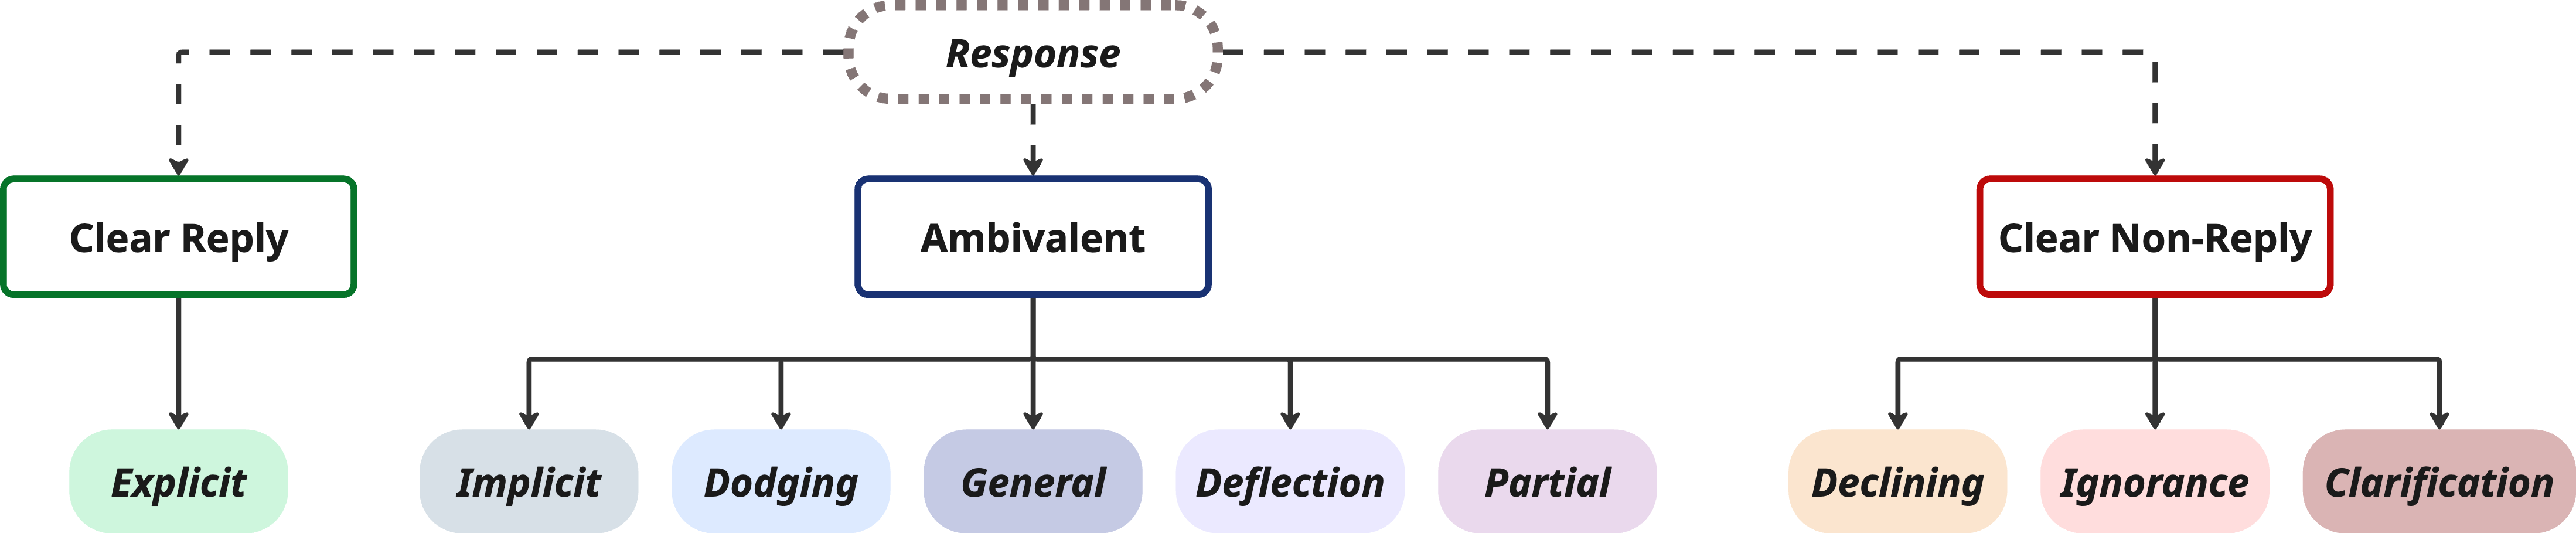
\includegraphics[width=\columnwidth]{assets/evasion-mapping.png}
\caption{Taxonomy: three clarity labels map to nine fine-grained evasion techniques \citep{thomas2024isaidthatdataset}.}
\label{fig:taxonomy}
\end{figure}

\subsection{Related Work}

\paragraph{Evasion Detection.}
\citet{thomas2024isaidthatdataset} introduce the QEvasion dataset and provide baselines for response clarity classification, building the foundation for the SemEval challenge.

\paragraph{LLM Prompting and Classification.}
\citet{brown2020language} demonstrate few-shot capabilities of large language models.
\citet{wei2022chain} show that chain-of-thought prompting improves reasoning and overall LLM performance.
\citet{sun2023textclassification} introduce a reasoning strategy to address the complex linguistic phenomena involved in text classification.

\paragraph{Prompt Optimization.}
OPRO \citep{yang2023opro} uses LLMs as optimizers with score-based feedback.
ProTeGi \citep{pryzant2023protegi} applies textual gradients for prompt refinement.
Our approach differs by using \emph{error-driven diagnosis} on concrete misclassified examples with structured failure-mode analysis, rather than abstract score optimization.


%% ===
%% 3 SYSTEM OVERVIEW
%% ===
\section{System Overview}

\subsection{Pipeline Architecture}

Our system is a Java-based end-to-end pipeline (Figure~\ref{fig:pipeline}) with four stages: \emph{Initialize} (load configuration, taxonomy, prompt template), \emph{Setup} (import data into Neo4j graph database, inject prompt data), \emph{Classify} (LLM calls with structured JSON output), and \emph{Evaluate} (compare results against the ground truth).

\begin{figure}[htbp]
\centering

\includegraphics[width=\columnwidth]{assets/pipeline.png}
\caption{End-to-end classification pipeline. YAML configuration files define taxonomy, prompt template, and model.}
\label{fig:pipeline}
\end{figure}

The pipeline is configuration-driven: YAML files specify the taxonomy, prompt template, LLM provider, and strategy.
We support four LLM providers: OpenAI, Anthropic, Together.ai, and local models. The classification is parallelized via a configurable thread pool.
Neo4j serves as the backend for provenance tracking and result storage.

\subsection{Classification Approach}
\label{sec:classification}

Our prompt template follows a structured design: role assignment, taxonomy with category descriptions, one few-shot example per category, interview context, question, and a JSON output format specification with the category name, an explanation, and a confidence score.

\begin{figure}[htbp]
\centering
\small
\begin{tcolorbox}[colback=blue!3,colframe=blue!70,title={\scriptsize\textbf{Input: QA Pair}},fonttitle=\sffamily,boxrule=0.4pt,left=3pt,right=3pt,top=2pt,bottom=2pt]
\scriptsize
\textbf{Q:} Do you see a risk of triggering a wider war?\\
\textbf{A:} I thought you were going to ask me about the pig.
\end{tcolorbox}
\vspace{1pt}
{\scriptsize$\Downarrow$\quad\textsf{LLM}}
\vspace{1pt}
\begin{tcolorbox}[colback=purple!3,colframe=purple!70,title={\scriptsize\textbf{Output: JSON Response}},fonttitle=\sffamily,boxrule=0.4pt,left=3pt,right=3pt,top=2pt,bottom=2pt]
\scriptsize\ttfamily
\{\\
\quad"name": "Dodging",\\
\quad"explanation": "The interviewer asks directly whether there \\
\quad\phantom{"explanation": "}is a risk of triggering a wider war. The\\
\quad\phantom{"explanation": "}interviewee does not address (...)",\\
\quad"confidence": 0.85\\
\}
\end{tcolorbox}
\vspace{1pt}
{\scriptsize$\Downarrow$\quad\textsf{Taxonomy Mapping}}
\vspace{1pt}
\begin{tcolorbox}[colback=gray!5,colframe=gray!50,boxrule=0.4pt,left=3pt,right=3pt,top=2pt,bottom=2pt]
\centering\scriptsize
\textsf{Dodging}~$\rightarrow$~\textsf{Ambivalent}
\end{tcolorbox}
\caption{Classification example: a QA pair is classified by the LLM, which returns a structured JSON response. The predicted evasion technique is mapped to its corresponding clarity label.}
\label{fig:classification-example}
\end{figure}

\paragraph{Evasion-based Mapping.}
Following the hierarchical taxonomy introduced by \citet{thomas2024isaidthatdataset}, we classify on the finer-grained 9-category evasion-technique level instead of directly predicting the 3 coarse clarity labels.
Predictions are mapped back to clarity labels via the definition in the taxonomy configuration (e.g., \emph{Deflection}~$\rightarrow$~\emph{Ambivalent}).
This approach consistently improves clarity performance (Section~\ref{sec:results}).

\subsection{Iterative Prompt Repair}
\label{sec:prompt-repair}

Our main contribution is an iterative prompt repair loop (Figure~\ref{fig:prompt-enhancer}) that systematically improves the prompt used for classification through error-driven diagnosis.

\begin{figure}[htbp]
\centering
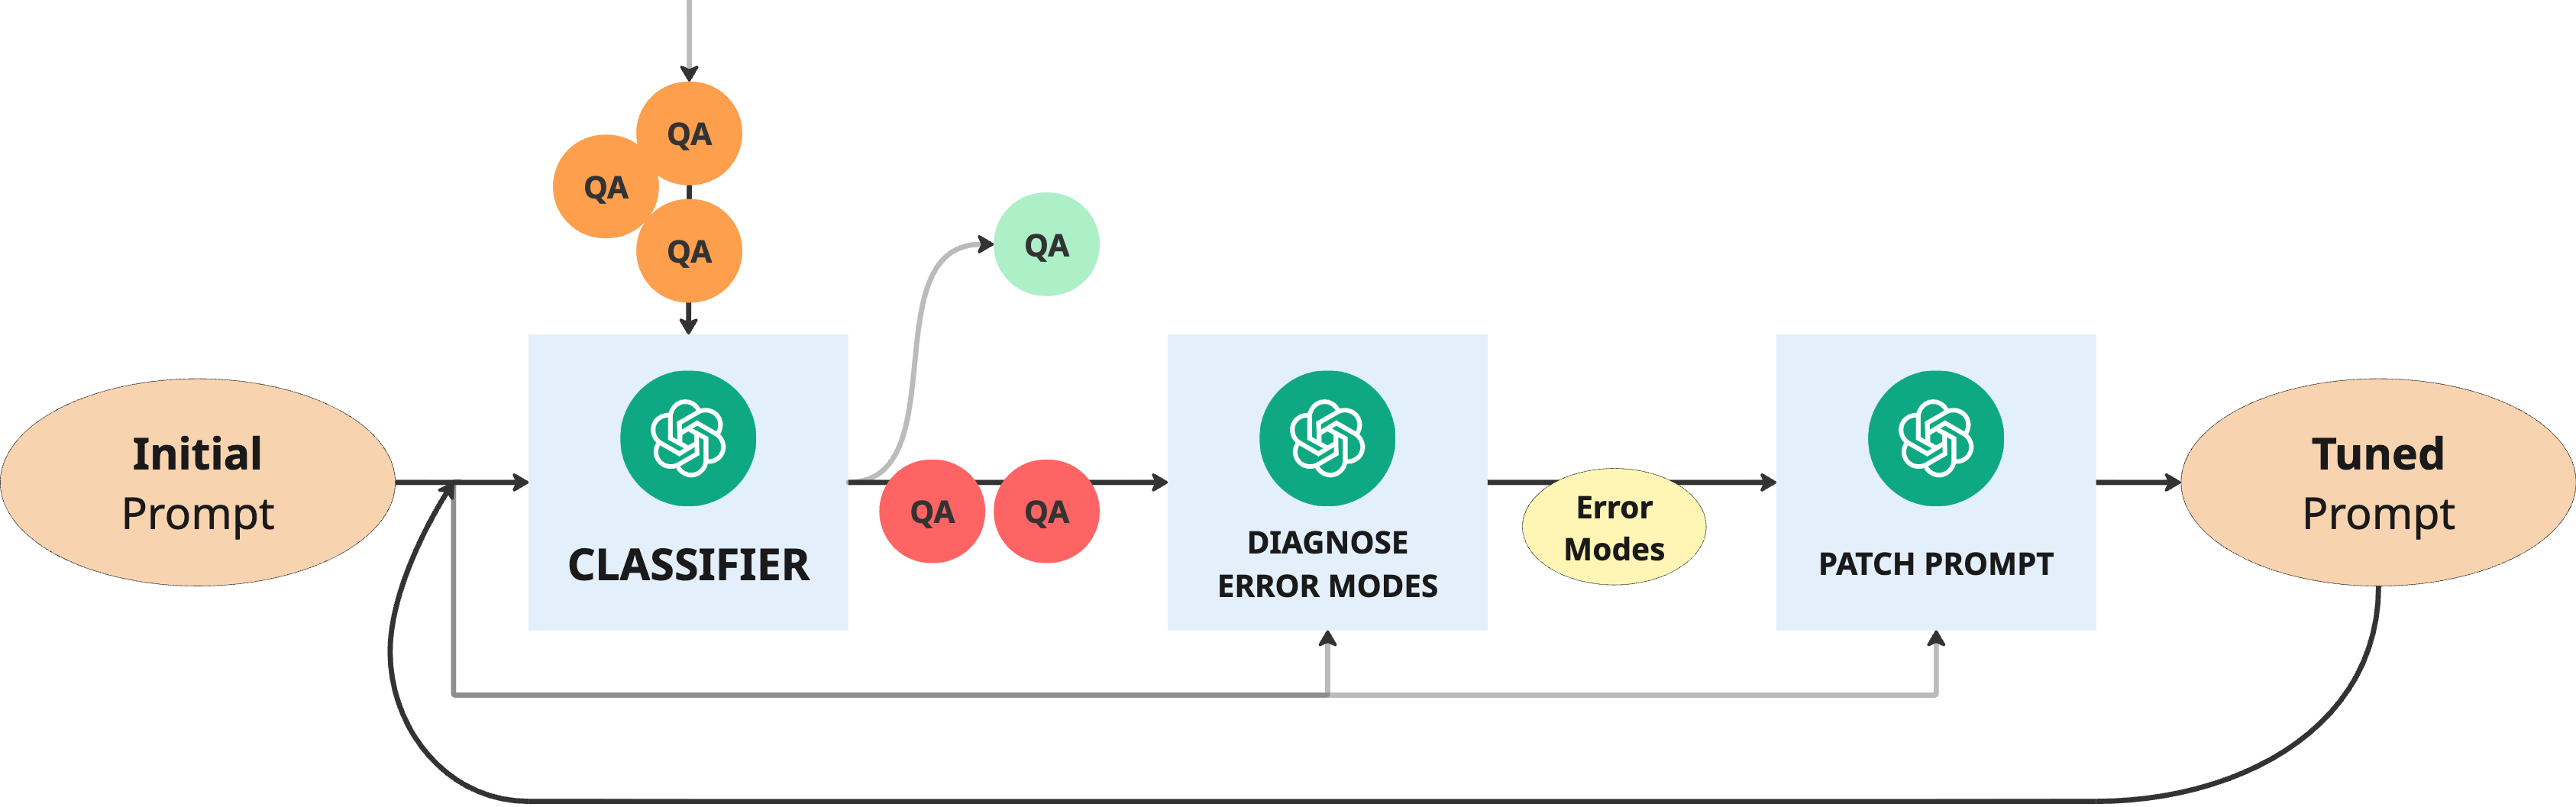
\includegraphics[width=\columnwidth]{assets/prompt-enhancer.png}
\caption{Iterative prompt repair: classify a sample, diagnose error modes from failures, and patch the prompt. The cycle repeats for $N$ iterations.}
\label{fig:prompt-enhancer}
\end{figure}

Each iteration consists of three phases:
\begin{enumerate}[nosep,leftmargin=*]
    \item \textbf{Classify:} Classify a sample of $N$ unseen training QA pairs with the current prompt and compare predictions against ground truth.
    \item \textbf{Diagnose Error Modes:} Feed misclassified examples (question, answer, predicted label, expected label, model explanation) to a diagnostic LLM prompt. The output is a set of failure modes, each with a name, description, and \emph{prompt drivers}, the specific lines in the current prompt that cause the error along with an explanation why the error was caused by that line.
    \item \textbf{Patch Prompt:} A separate LLM call receives the failure modes and current prompt, then generates a revision.
\end{enumerate}

The diagnosis and patching steps are deliberately separated to reduce overfitting: diagnosis identifies systematic patterns across multiple failures, while the patch addresses these patterns with generalizable prompt revisions rather than example-specific fixes.

{\raggedright
\paragraph{Example.}
Figure~\ref{fig:prompt-repair-example} illustrates one repair iteration from iteration~1.
The diagnostic step identifies the failure mode:

\noindent\texttt{overly\_narrow\_definition\_of\_dodging}

\noindent the base prompt defines Dodging as \emph{``ignoring the question altogether,''} which is too general.
The patch broadens the definition for Dodging.
\par}

\begin{figure}[htbp]
\centering
\small
\begin{tcolorbox}[colback=orange!3,colframe=orange!80,title={\scriptsize\textbf{1.\ Diagnose: Failure Mode}},fonttitle=\sffamily,boxrule=0.4pt,left=3pt,right=3pt,top=2pt,bottom=2pt]
\scriptsize
\textbf{Mode:} \texttt{overly\_narrow\_definition\_of\_dodging}\\[2pt]
\textbf{Prompt driver:} \emph{``Dodging: ignoring the question altogether''}\\
\textbf{Description:} The prompt’s 'dodging' definition is too narrow, and does not define a key real-world pattern: responding with adjacent context while never providing the requested fact (...)\\[2pt]
\end{tcolorbox}
\vspace{1pt}
{\scriptsize$\Downarrow$\quad\textsf{Patch Prompt}}
\vspace{1pt}
\begin{tcolorbox}[colback=cyan!3,colframe=cyan!80,title={\scriptsize\textbf{2.\ Prompt Revision}},fonttitle=\sffamily,boxrule=0.4pt,left=3pt,right=3pt,top=2pt,bottom=2pt]
\scriptsize
\textbf{Before:} \emph{``Dodging: Ignoring the question altogether.''}\\[2pt]
\textbf{After:} \emph{``Dodging: Does not answer the core request; may talk around it or provide adjacent/related context, but never provides the asked-for information.''}\\[2pt]
\end{tcolorbox}
\caption{Prompt repair example (iteration~1): the diagnostic step identifies a failure mode with specific prompt drivers. The patch adjusts the prompt.}
\label{fig:prompt-repair-example}
\end{figure}

\subsection{Data Preprocessing}
We implement a 5-step preprocessing pipeline (Figure~\ref{fig:preprocessing-pipeline}):
(1)~spelling correction (NLTK\footnote{\url{https://www.nltk.org/}}, RapidFuzz\footnote{\url{https://github.com/rapidfuzz/RapidFuzz}, v3.14.3}, wordfreq\footnote{\url{https://github.com/rspeer/wordfreq}, v3.1.1}),
(2)~word-spacing repair (WordNinja\footnote{\url{https://github.com/keredson/wordninja}, v2.0.0}),
(3)~optional removal of names and identifiers,
(4)~optional removal of filler words and phrases (spaCy\footnote{\url{https://spacy.io}, v3.8.11}; \citealt{honnibal2020spacy}), and
(5)~punctuation normalization.

\begin{figure}[htbp]
    \centering
    \includegraphics[width=\columnwidth]{latex/assets/preprocessing-pipeline.png}
    \caption{Five-stage preprocessing pipeline}
    \label{fig:preprocessing-pipeline}
\end{figure}

Although preprocessing improves subjective data quality, it does not yield consistent metric gains (Section~\ref{sec:results}), suggesting that relevant signals (e.g. fillers, hedging markers) may be removed by aggressive cleaning.

%% ===
%% 4 EXPERIMENTAL SETUP
%% ===
\section{Experimental Setup}

\paragraph{Dataset.}
We use the QEvasion dataset \citep{qevasion2024}, consisting of English-language political interviews of US-Presidents.
We report all metrics on the test set (308 QA pairs) using the provided ground-truth labels.

\paragraph{Models.}
Our primary model is GPT-5.2 \citep{openai2025gpt52}.
We compare against GPT-5.1 \citep{openai2025gpt51}, GPT-5 \citep{openai2025gpt5}, GPT-4.1 \citep{openai2025gpt41}, o3, GPT-5-Nano, Claude~Sonnet~4.5 \citep{anthropic2025claude45}, Llama~3.3~70B \citep{meta2024llama3}, GPT-OSS-120B \citep{openai2025gptoss}, Kimi-K2-Thinking \citep{moonshot2025kimi}, and Llama~3.1~8B \citep{meta2024llama} as open-source baseline.

\paragraph{Configurations.}
We evaluate 70+ configurations across 5 strategy families:
(1)~Direct clarity classification,
(2)~Evasion-based mapping,
(3)~RAG with embedding-based example retrieval,
(4)~Prompt iteration pipeline (12 iterations with GPT-5.2), and
(5)~Alternative approaches with cleaned data, reasoning-effort settings, and PAG \citep{yadav2024pag}.

\paragraph{Metrics.}
We report accuracy and macro~F1 as the primary metrics for both sub-tasks.

\paragraph{Hyperparameters.}
We use \texttt{max\_tokens=4096} with structured JSON output.
GPT-5 family models do not support user-configurable temperature.
We apply 3 retry attempts with exponential backoff.
For prompt enhancement, we run 12 iterations with 20 randomly sampled training examples per iteration using GPT-5.2 for classification, diagnosis, and patching.
The iteration with the best performance is selected post-hoc based on the metrics of the test dataset; no stopping criterion was applied during the run.

%% ===
%% 5 RESULTS
%% ===
\section{Results}
\label{sec:results}

\paragraph{Main Results.}
Table~\ref{tab:main} presents key configurations.
Evasion-based mapping yields +5.8pp clarity accuracy and +6.8pp clarity F1 over direct classification.
Iterative prompt repair further improves Evasion~F1 by +13.7pp (0.438$\rightarrow$0.575) while maintaining clarity performance.
The best evasion result (It.~7: 0.620~Acc~/~0.575~F1) comes at iteration 7, while the best clarity result (It.~8: 0.831~Acc~/~0.797~F1) is at iteration 8.

\begin{table}[htbp]
\centering
\small
\begin{tabular}{@{}lcccc@{}}
\toprule
\textbf{Configuration} & \multicolumn{2}{c}{\textbf{Clarity}} & \multicolumn{2}{c}{\textbf{Evasion}} \\
\cmidrule(lr){2-3} \cmidrule(lr){4-5}
 & Acc & F1 & Acc & F1 \\
\midrule
Llama 3.1 8B (Baseline) & .685 & .451 & .312 & .182 \\
GPT-5.2 (Direct) & .773 & .708 & -- & -- \\
GPT-5.2 (Evasion Map) & .831 & .776 & .477 & .438 \\
GPT-5.2 (It.~7)$^\ddagger$ & .808 & .780 & \textbf{.620} & \textbf{.575} \\
GPT-5.2 (It.~8)$^\dagger$ & \textbf{.831} & \textbf{.797} & .614 & .574 \\
\bottomrule
\end{tabular}
\caption{Key configurations. $^\dagger$Best clarity. $^\ddagger$Best evasion. Direct = clarity-only taxonomy; Evasion Map = evasion-based mapping; It.~$n$ = prompt repair iteration~$n$.}
\label{tab:main}
\end{table}

\paragraph{Model Comparison.}
Table~\ref{tab:models} compares models using evasion-based mapping without prompt enhancement.
Frontier models (GPT-5.x) dominate clarity, while GPT-5 and o3 show stronger evasion performance despite lower clarity scores.
Smaller open-source models lag substantially: Llama~3.1~8B achieves only 0.451~F1 (clarity), though Llama~3.3~70B is more competitive at 0.636~F1, indicating that model size and architecture are important factors for this task.

\begin{table}[htb]
\centering
\small
\begin{tabular}{@{}lcccc@{}}
\toprule
\textbf{Model} & \multicolumn{2}{c}{\textbf{Clarity}} & \multicolumn{2}{c}{\textbf{Evasion}} \\
\cmidrule(lr){2-3} \cmidrule(lr){4-5}
 & Acc & F1 & Acc & F1 \\
\midrule
GPT-5.2 & \textbf{.831} & \textbf{.776} & .477 & .438 \\
GPT-5.1 & .808 & .776 & .552 & .488 \\
GPT-4.1 & .812 & .758 & .500 & .498 \\
GPT-5 & .763 & .727 & \textbf{.614} & \textbf{.548} \\
o3 & .731 & .726 & .607 & .529 \\
Claude Sonnet 4.5 & .750 & .659 & .442 & .421 \\
Llama 3.3 70B & .753 & .636 & .406 & .414 \\
GPT-OSS-120B & .763 & .707 & .516 & .439 \\
Kimi-K2-Thinking & .786 & .699 & .435 & .409 \\
GPT-5-Nano & .679 & .662 & .500 & .419 \\
Llama 3.1 8B & .688 & .475 & .312 & .182 \\
\bottomrule
\end{tabular}
\caption{Model comparison using evasion-based mapping (no prompt enhancement). Best per column in \textbf{bold}.}
\label{tab:models}
\end{table}

\paragraph{Prompt Repair Convergence.}
Figure~\ref{fig:convergence} shows F1 progression across 12 prompt repair iterations using a sample of 20 training examples per iteration.
Evasion~F1 improves substantially (+13.7pp overall) with a clear upward trend, while clarity~F1 remains relatively stable with non-monotone fluctuations.
We attribute the non-monotone behavior primarily to the small sample size per iteration: Since only 20 randomly selected training examples are used, the number of observed failures varies across iterations, introducing noise in the diagnostic signal that causes individual patches to occasionally degrade performance in cases that were previously handled well.

\begin{figure}[htb]
\centering
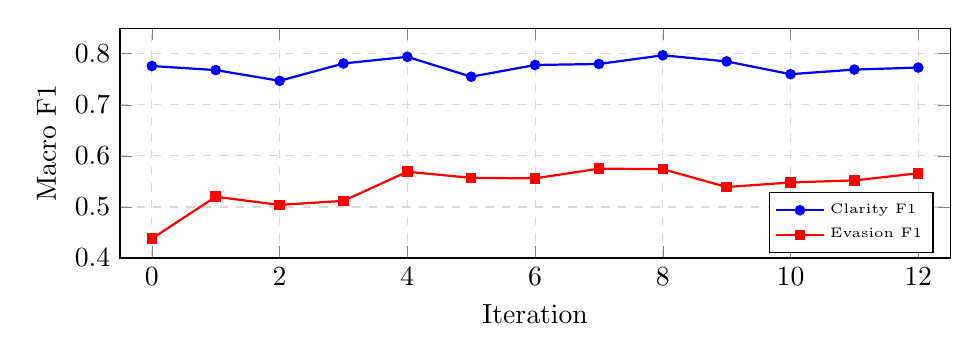
\begin{tikzpicture}
\begin{axis}[
    width=\columnwidth,
    height=4.5cm,
    xlabel={Iteration},
    ylabel={Macro F1},
    xmin=-0.5, xmax=12.5,
    ymin=0.40, ymax=0.85,
    xtick={0,2,...,12},
    ytick={0.40,0.50,0.60,0.70,0.80},
    legend style={at={(0.98,0.02)},anchor=south east,font=\tiny,legend cell align=left,row sep=0pt,inner sep=2pt},
    grid=major,
    grid style={dashed,gray!30},
    mark size=1.5pt,
]
\addplot[blue, mark=*, thick] coordinates {
    (0,0.776) (1,0.768) (2,0.747) (3,0.781) (4,0.794)
    (5,0.755) (6,0.778) (7,0.780) (8,0.797) (9,0.785)
    (10,0.760) (11,0.769) (12,0.773)
};
\addlegendentry{Clarity F1}
\addplot[red, mark=square*, thick] coordinates {
    (0,0.438) (1,0.520) (2,0.504) (3,0.512) (4,0.569)
    (5,0.557) (6,0.556) (7,0.575) (8,0.574) (9,0.539)
    (10,0.548) (11,0.552) (12,0.566)
};
\addlegendentry{Evasion F1}
\end{axis}
\end{tikzpicture}
\caption{Macro F1 over prompt repair iterations. Evasion F1 shows clear improvement; Clarity F1 remains stable with non-monotone fluctuation.}
\label{fig:convergence}
\end{figure}

\paragraph{RAG and Alternative Strategies.}
RAG with embedding-based example retrieval yields inconsistent results.
PAG \citep{yadav2024pag} (paraphrasing questions, classifying each one and aggregating results through a majority vote) shows a similar performance to single-shot classification (GPT-5.1: 0.812~Acc~/~0.789~F1).
Setting reasoning effort to ``high'' had no clear effect. Some models performed better, others worse than without it.
Applying the enhanced prompt to cleaned data degrades performance (0.831/0.797~$\rightarrow$~0.812/0.716 clarity Acc/F1), suggesting that aggressive preprocessing removes relevant signals such as fillers and hedging markers. Identifying which specific steps are responsible requires further investigation.

%% ===
%% 6 CONCLUSION
%% ===
\section{Conclusion}

We presented an LLM-first pipeline for detecting political question evasion with two core contributions: an iterative prompt repair loop via error-driven diagnosis, and a configurable multi-provider pipeline enabling systematic experimentation.
Leveraging the hierarchical taxonomy of \citet{thomas2024isaidthatdataset}, we classify at the fine-grained level and map back to clarity labels, consistently improving performance.
Our system achieves 0.831 accuracy / 0.797 macro~F1 on clarity classification and 0.620 accuracy / 0.575 F1 on evasion techniques, improving over \citet{thomas2024isaidthatdataset} by +11.8pp accuracy and +11.5pp F1 on clarity.

\paragraph{Limitations.}
(1)~Our system relies on API-based models, introducing cost, latency, and reproducibility constraints.
(2)~Prompt repair convergence is non-monotone, and the best-performing iteration is selected post-hoc without a principled stopping criterion.
A validation-set-based early stopping strategy would reduce overfitting risk and cost, but requires further development.
(3)~Local baselines are limited; no full fine-tuning was evaluated.
(4)~Preprocessing the data did not translate into clear and consistent metric improvements; which specific cleaning steps remove diagnostically relevant signals remains an open question.

\paragraph{Future Work.}

First, we aim to broaden the set of reproducible local baselines. This includes incorporating fine-tuned encoder-based models as well as stronger open-source LLM baselines. In addition, we plan to conduct systematic ablation studies to more clearly isolate and quantify the contribution of individual components of the system.
Second, we intend to treat preprocessing as a tunable policy. By systematically exploring different combinations of cleaning and normalization steps, we seek to identify configurations that improve robustness and generalization across datasets and domains.
Third, we plan to develop a principled stopping criterion for the prompt enhancement pipeline.
Specifically, evaluating each iteration on a held-out validation split instead of post-hoc on the test set would allow for unbiased iteration selection. This would also enable early stopping once performance gains plateau, which would reduce cost and the risk of overfitting to the sampled failure cases.

%% ===
%% BIBLIOGRAPHY
%% ===
% Bibliography entries for the entire Anthology, followed by custom entries
% \bibliography{anthology,custom}
% Custom bibliography entries only
\bibliography{custom}

%% ===
%% APPENDIX
%% ===
\appendix

\section{Taxonomy Definitions}

Table~\ref{tab:taxonomy} presents the complete 9-category evasion-technique taxonomy of \citet{thomas2024isaidthatdataset} with descriptions, clarity mappings, and representative examples.

\begin{table*}[htbp]
\centering
\small
\begin{tabular}{@{}p{2.2cm}p{3.8cm}p{1.8cm}p{3.0cm}p{3.5cm}@{}}
\toprule
\textbf{Category} & \textbf{Description} & \textbf{Maps to} & \textbf{Example Q} & \textbf{Example A} \\
\midrule
Explicit & The information requested is explicitly stated in the requested form & Clear Reply & Do you have your own views about PR? & I do. \\
\addlinespace
Implicit & The information is given but not explicitly stated & Ambivalent & Are you going to watch television? & What else is there to do? \\
\addlinespace
General & The information provided is too general / lacks specificity & Ambivalent & What's your favorite film? & Fight Club, Filth, and Hereditary. \\
\addlinespace
Partial/half-answer & Offers only a specific component of the requested information & Ambivalent & Did you enjoy the film? & The directing was great. \\
\addlinespace
Dodging & Ignoring the question altogether & Ambivalent & Do you like my new dress? & We are late. \\
\addlinespace
Deflection & Starts on topic but shifts focus to a different point & Ambivalent & Did you eat the last piece of pie? & I have to admit that this was a great recipe\ldots \\
\addlinespace
Declining to answer & Acknowledges the question but refuses to answer & Clear Non-Reply & Wouldn't you regard that as a defeat? & I am not going to prophesy what will happen. \\
\addlinespace
Claims ignorance & Claims not to know the answer & Clear Non-Reply & On what precise date did\ldots? & I do not know that date. \\
\addlinespace
Clarification & Asks for clarification instead of answering & Clear Non-Reply & Was it your decision to release the fund? & You mean the public fund? \\
\bottomrule
\end{tabular}
\caption{Complete evasion-technique taxonomy with mapping from evasion techniques to clarity categories \citep{thomas2024isaidthatdataset}.}
\label{tab:taxonomy}
\end{table*}

\section{Prompt Templates}
\label{sec:appendix-prompts}

\subsection{Base Classification Prompt}
\label{sec:appendix-base-prompt}

The base prompt used before iterative refinement:

\begin{lstlisting}[style=yaml]
You are an expert in political sciences and interview analysis.
Your task is to classify the type of responses given by interviewees
based on the questions posed by the interviewer.

Based on a segment of the interview in which the interviewer poses a
series of questions, classify the type of response provided by the
interviewee for the following question using the following taxonomy and
then provide a chain of thought explanation for your decision:

1. Explicit - The information requested is explicitly...
[... rest of the techniques and descriptions ...]

---
Here is one small example for each term of the taxonomy:

[... one example for all 9 categories ...]
---

Here is the segment of the interview that you should analyze:

**Part of the Interview**
[... context of the interview ...]

**Question**
[... question ...]

**Output**
Respond with a JSON object in the following format:
{
"name": <STRING | Name of the classified category>,
"explanation": <STRING | Explanation for the classification decision>,
"confidence": <DOUBLE | Confidence score between 0 and 1 inclusive>
}
\end{lstlisting}

\subsection{Enhanced Prompt (Iteration 8)}
\label{sec:appendix-enhanced-prompt}

The enhanced prompt after 8 iterations of prompt repair:

\begin{lstlisting}[style=yaml]
You are an expert in political sciences and interview analysis.
Your task is to classify the type of responses given by interviewees based
on the questions posed by the interviewer.

Based on a segment of the interview in which the interviewer poses a series
of questions, classify the type of response provided by the interviewee for
the following question using the following taxonomy and then provide a brief,
evidence-based explanation for your decision (1–3 sentences). Quote or
paraphrase the key phrase(s) that justify the label.

Taxonomy (category names must be used exactly):
[... refined description for all 9 categories ...]

Decision rules (apply in order):

1) Identify the “requested variable” (slot)
- Identify exactly what specific information the question requests (the
“requested variable”), including each explicit sub-part, condition, timeframe,
or forced-choice option. Treat this as a concrete slot that must be filled
(e.g., a specific yes/no, named choice, actor, date/number, stance, or action).

2) Check for a slot-fill FIRST (hard precedence)
- Before considering General/Dodging/Deflection, scan the entire response
  for ANY clear commitment that fills the requested slot at the specificity
  level demanded.
  - If all explicitly requested parts/conditions are filled → Explicit
    (or Implicit if only inferable under rule 5).
  - If some (but not all) explicitly requested parts/conditions are filled
    → Partial/half-answer.
- Only if there is NO clear slot-fill anywhere should you choose among General
  /Dodging/Deflection (or Declining/Claims ignorance/Clarification).

3) What counts as a slot-fill (and what does NOT)
- Count as answering only if the response fills the slot with a clear commitment
  at the same specificity level the question demands.
  - Do NOT treat as answering: mere topic alignment, reassurance, rhetorical
    soothing, slogans, broad principles, policy/process descriptions, meta-
    commentary about discussion, future intent (“we’ll look at it”), promises
    to decide later, or conditional/hedged non-commitments (“it depends,” “we’ll
    see,” “in due course”), unless they STILL clearly commit to a particular
    value/side now.
  - Specificity match: If the question asks for concrete details (e.g., who/what
    /when/which terms/what exactly was said), then abstract aspirations, broad
    principles, or “we discussed X” without the requested specifics are NOT an
    answer.
  - Reframing is not automatically an answer: A response may reject the premise
    or reframe and STILL answer—but only if it clearly commits to the requested
    slot value/side.

4) Declining / ignorance / clarification detection (before General/Dodging/Deflection)
- If the response includes refusal/constraint language, label Declining to answer
  UNLESS the speaker nevertheless provides the requested slot value at the required
specificity.
  - Treat “soft” political constraints as Declining to answer when they function as
    non-disclosure (e.g., “I can’t get into that,” “I’m not going to talk about that,”
    “we keep that close to the vest,” “it’s not appropriate to discuss details,”
    “I’m not at liberty”).
  - If refusal/constraint is followed by generic positivity/progress talk, do NOT
    upgrade to Explicit/Implicit unless the slot is actually filled.
- Use Claims ignorance when the speaker indicates lack of knowledge/awareness/
  certainty about the requested variable (including “I don’t know,” “I’m not aware,”
  “I haven’t seen,” “I don’t have that information,” “I’m not sure,” “as far as I know,”
  “I assume,” “I’ve heard,” or other language that signals they cannot vouch for the
  asked-for fact).
- Use Clarification if the response is a genuine question needed to understand what
  is being asked and does not yet provide the requested information.

5) Implicit (use narrowly, but do not miss real commitments)
- Use Implicit ONLY when the response leaves only one materially plausible value/side
  for the requested slot.
  - If the statement could reasonably fit multiple values/sides (e.g., reassurance,
    optimism, “we’re working on it,” “we take it seriously,” “we’re making progress,”
    “we’ll review”), do NOT label Implicit.
  - In those cases: use General (if they are trying to give the slot value but it
    stays vague) or Dodging/Deflection (if they avoid giving the slot value).
- Explicit vs Implicit guardrail: Explicit requires the slot value be directly stated
  at the demanded granularity; if the slot value is only obtained by inference (even
  strong inference), it is Implicit, not Explicit.

6) Forced-choice / yes-no / evaluative questions
- For forced-choice or yes/no questions: the response must clearly commit to one side
  (Explicit OR Implicit under rule 5). Non-committal hedging (“maybe/it depends/we’ll
  decide later”) is not an answer.
- For evaluative yes/no asks (e.g., “is there a problem?”, “should people worry?”,
  “was that a mistake?”): citing related facts, describing efforts, or expressing
  confidence/concern does NOT automatically equal “yes” or “no” unless the speaker
  actually makes that judgment.

7) Multi-part, conditional, and list/boundary questions
- Explicit = all explicitly requested parts/conditions are answered with clear
  commitments.
- Partial/half-answer = at least one explicitly requested part/condition is answered
  with a clear commitment, but not all.
- Guardrail (avoid Partial overuse): If the question asks for actions/measures/steps
  and does NOT explicitly require an exhaustive list (or explicitly require both sides
  such as “what will you do” AND “what won’t you do”), then providing one concrete
  committed measure can be sufficient for Explicit.
- If the speaker answers a different condition/version than asked (e.g., answers “with
  a deal” while avoiding the asked “if no deal by date”), treat that as Deflection
  unless they also clearly commit on the asked condition.

8) If none of the requested parts are answered: choose General vs Dodging vs Deflection
- General = the speaker is trying to answer the same requested slot (attempting to
  provide the value/side) but the value remains too vague/underspecified to fill it.
- Deflection = the speaker substitutes a different proposition/variable as the main
  answer OR explicitly pivots to a new agenda/main claim that could stand alone as what
  they want to talk about instead of answering the slot (often signaled by “the real
  issue is…,” “what matters is…,” attacking the questioner/premise, or switching to
  broader messaging). If they still clearly fill the slot, do NOT use Deflection.
- Dodging = the speaker does not fill the slot and does not clearly substitute a
  different proposition as the main answer; includes stalling, meandering adjacent
  remarks, or on-topic context that never supplies the requested value.

9) Evidence requirement (keep it tight)
- In 1–3 sentences (prefer 1–2 unless truly necessary), quote or paraphrase the
  single strongest phrase(s) that contain the slot-fill (Explicit/Implicit/Partial)
  OR the refusal/ignorance/clarifying question/pivot/vagueness (Declining/Claims
  ignorance/Clarification/Deflection/General/Dodging).

---
Here is one small example for each term of the taxonomy:

[... refined examples for all 9 categories ...]

---
Additional targeted guardrail examples:

Question: Should people be worried about X?
Answer: We’re working around the clock and we have this under control.
Label: Dodging
Explanation: Reassurance does not explicitly or unambiguously answer “yes/no”
  to whether people should be worried.

Question: Will you resign?
Answer: I’m focused on delivering for the public; we’ll review matters
  in due course.
Label: Dodging
Explanation: Future-intent/process language does not commit to “yes” or “no.”

Question: Did you approve the report?
Answer: You should ask the department / read the report.
Label: Declining to answer
Explanation: Directing elsewhere substitutes for answering.

Question: Did the administration sanction torture?
Answer: Waterboarding was torture.
Label: Deflection
Explanation: The speaker answers a different proposition (a moral/definitional
  claim) instead of the requested yes/no about sanctioning.

---
Here is the segment of the interview that you should analyze:

**Part of the Interview**
[... context of the interview ...]

**Question**
[... question ...]

**Output**
Respond with a JSON object in the following format:
{
  "name": <STRING | Name of the classified category>,
  "explanation": <STRING | Explanation for the classification decision>,
  "confidence": <DOUBLE | Confidence score between 0 and 1 inclusive, up to two decimals.>
}
\end{lstlisting}

\subsection{Diagnose Prompt}
\label{sec:appendix-diagnose}

\begin{lstlisting}[style=yaml]
You are a prompt engineer tasked with debugging a prompt for a classification
pipeline that classifies the type of responses given by interviewees based on
the questions posed by the interviewer.

You are given:

1) The current prompt:
<prompt>
{dump_prompt}
</prompt>

2) A small set of logged failures. Each log has:
- query
- model_answer
- expected_answer

<failure_traces>
{dump_failure_traces}
</failure_traces>

Your tasks:

1) Identify the distinct failure mode you see (e.g., misunderstanding_of_taxonomy,
   insufficient_context_utilization, lack_of_chain_of_thought).
2) For each failure mode, quote or paraphrase the specific lines or sections of
   the prompt that are most likely causing or reinforcing it. Include any contradictions.
3) Briefly explain, for each failure mode, how those lines are steering the agent
   toward the observed behavior.

Respond with a JSON object in the following format:
{
    "name": <STRING | Name of the failure mode>,
    "description": <STRING | Description of the failure mode>,
    "prompt_drivers": [
        {
            "exact_or_paraphrased_line": <STRING | Exact or paraphrased line from the prompt>,
            "why_it_matters": <STRING | Explanation why this line is a driver for the failure mode>
        }
    ]
}
\end{lstlisting}

\subsection{Patch Prompt}
\label{sec:appendix-patch}

\begin{lstlisting}[style=yaml]
You previously analyzed this prompt and its failure modes.

1) Prompt:

  <prompt>
  {dump_prompt}
  </prompt>

  The prompt contains the following placeholders in square brackets:
  <placeholders>
    - context
    - question
  </placeholders>
  The placeholders are dynamically filled in at runtime and specific
  to the Question-Answer pair being classified.

2) Failure-mode analysis:
  <failure-mode-analysis>
  {dump_failure_mode_analysis}
  </failure-mode-analysis>

  Please propose a surgical revision of the prompt that reduces the
  observed issues while preserving the good behaviors.

**Constraints:**

  - Do not redesign the agent from scratch.
  - Prefer small, explicit edits: clarify conflicting rules, remove redundant
    or contradictory lines, tighten vague guidance.
  - Make tradeoffs explicit (for example, clearly state when to prioritize
    concision over completeness).
  - The names of the taxonomy categories MUST remain unchanged.
  - The response format MUST remain unchanged.
  - The runtime placeholders (in square brackets) are immutable and must remain
    verbatim. Treat them as non-editable tokens.
  - Do NOT mention, reference, describe, or explain placeholders by name anywhere
    else in the prompt text. When giving instructions about their content, refer
    to them indirectly, e.g. "the interview segment", "the provided question", etc.

**Output:**

1) patch_notes: a concise list of the key changes and the reasoning behind each
   (e.g., "Instruction X was ambiguous and led to Y; revised to Z to clarify intent").
2) revised_prompt: the full updated prompt with your edits applied, ready to drop
   into an agent configuration and all placeholders intact.

Respond with a JSON object in the following format:
{
    "revised_prompt": <STRING | The revised prompt after applying the patches>,
    "patch_notes": [
        <STRING | Note describing a specific change made in the patch>,
        ...
    ]
}
\end{lstlisting}

\section{Configuration Examples}
\label{sec:appendix-config}

\subsection{Classification Run}
\label{sec:appendix-classification-config}

Example configuration for a single-model evasion-based classification run:

\begin{lstlisting}[style=yaml]
name: "GPT 5.2"
version: "evasion-based:single:few-shot:v1"
taxonomy: "../assets/taxonomy/evasion-techniques.yaml"
worker-threads: 50
query: |
  MATCH (n:QA)
  WHERE n.test = true
  RETURN n
strategy:
  type: "single"
  model:
    provider: "openai"
    name: "gpt-5.2"
    prompt: "../assets/prompts/few-shot.yaml"
\end{lstlisting}

\subsection{Prompt Enhancement Run}
\label{sec:appendix-prompt-enhancement-config}

Configuration for the iterative prompt repair pipeline:

\begin{lstlisting}[style=yaml]
name: "GPT 5.2"
version: "prompt-enhancing:v3"
taxonomy: "../assets/taxonomy/evasion-techniques-no-mapping.yaml"
iterations: 12
n: 20
worker-threads: 50
save-temporary-results: true
classification-prompt: "../assets/prompts/prompt-enhancement/base.yaml"
enhancement-prompt-diagnose: "../assets/prompts/prompt-enhancement/diagnose.yaml"
enhancement-prompt-patch: "../assets/prompts/prompt-enhancement/patch.yaml"
output-prompt: "../assets/prompts/prompt-enhancement/gpt-5.2-v3-output.yaml"
query: |
  MATCH (n:QA)
  WHERE n.train = true
  RETURN n
model:
  provider: "openai"
  name: "gpt-5.2"
\end{lstlisting}

\subsection{Taxonomy Configuration}
\label{sec:appendix-taxonomy-config}

Taxonomy YAML configuration for the evasion techniques:

\begin{lstlisting}[style=yaml]
name: "Evasion Techniques"
version: "v1"
mapping:
  enabled: true
  label-property: "clarityLabel"
  labels:
    - "Clear Reply"
    - "Ambivalent"
    - "Clear Non-Reply"
label-property: "evasionLabel"
categories:
  - name: "Explicit"
    map-to: "Clear Reply"
    examples:
      - question: Do you have your own views about PR at Westminster don’t you?
        answer: I do.
        explanation: The answer directly gives the info requested.
    description: >
      The information requested is explicitly stated (in the requested form)
  - name: "Implicit"
    map-to: "Ambivalent"
    examples:
      - question: Are you going to watch television?
        answer: What else is there to do?
        explanation: They suggest planning to watch TV, despite not explicitly stating it.
    description: >
      The information requested is given, but without being explicitly stated
      (not in the expected form)
  - name: "General"
    map-to: "Ambivalent"
    examples:
      - question: What’s your favorite film?
        answer: Fight Club, Filth, and Hereditary.
        explanation: The reply gives three movies instead of one, which makes the desired information unclear.
    description: >
      The information provided is too general/lacks the requested specificity
  - name: "Partial/half-answer"
    map-to: "Ambivalent"
    examples:
      - question: Did you enjoy the film?
        answer: The directing was great.
        explanation: Directing is only part of what constitutes a film.
    description: >
      Offers only a specific component of the requested information
  - name: "Dodging"
    map-to: "Ambivalent"
    examples:
      - question: Do you like my new dress?
        answer: We are late.
        explanation: Does not even acknowledge the question and goes straight to another topic.
    description: >
      Ignoring the question altogether
  - name: "Deflection"
    map-to: "Ambivalent"
    examples:
      - question: Did you eat the last piece of pie?
        answer: I have to admit that this was a great recipe, I always like it when there are chocolate chips in the dough.
        explanation: Acknowledges the question but goes on a tangent about the chips, without answering.
    description: >
      Starts on topic but shifts the focus and makes a different point than what is asked
  - name: "Declining to answer"
    map-to: "Clear Non-Reply"
    examples:
      - question: The hypothesis I was discussing, wouldn’t you regard that as a defeat?
        answer: I am not going to prophesy what will happen.
        explanation: Directly stating they won’t answer.
    description: >
      Acknowledge the question but directly or indirectly refusing to answer
      at the moment
  - name: "Claims ignorance"
    map-to: "Clear Non-Reply"
    examples:
      - question: On what precise date did the government order the refit of the HMAS Kanimbla in preparation for its forward deployment to a possible war against Iraq?
        answer: I do not know that date. I will find out and let the House know.
        explanation: Claims or admits they don’t have the information.
    description: >
      The answerer claims/admits not to know the answer themselves
  - name: "Clarification"
    map-to: "Clear Non-Reply"
    examples:
      - question: Was it your decision to release the fund?
        answer: You mean the public fund?
        explanation: Gives no data, asks for clarification.
    description: >
      Does not provide the requested information and asks for clarification
\end{lstlisting}

\section{Full Result Tables}
\label{sec:appendix-results}

Table~\ref{tab:all-results} presents all 73 evaluated configurations grouped by strategy.
Clarity metrics are reported for all configurations; evasion metrics are only available for evasion-based runs.
All values are computed on the test set (308~QA pairs).

\begin{table*}[p]
\centering
\scriptsize
\begin{tabular*}{\textwidth}{@{\extracolsep{\fill}}llcccc@{}}
\toprule
\textbf{Group} & \textbf{Configuration} & \textbf{C.~Acc} & \textbf{C.~F1} & \textbf{E.~Acc} & \textbf{E.~F1} \\
\midrule
\multicolumn{6}{l}{\textbf{Direct Clarity Classification}} \\
\midrule
Normal & GPT-5.2 & .773 & .708 & -- & -- \\
 & Kimi-K2-Thinking & .773 & .689 & -- & -- \\
 & GPT-5 & .724 & .677 & -- & -- \\
 & GPT-OSS-120B & .708 & .651 & -- & -- \\
 & Claude Sonnet 4.5 & .705 & .609 & -- & -- \\
 & GPT-4.1 & .695 & .599 & -- & -- \\
 & GPT-5 Nano & .695 & .625 & -- & -- \\
 & Llama 3.3 70B & .695 & .553 & -- & -- \\
 & Llama 3.1 8B & .685 & .451 & -- & -- \\
 & GPT-5.1 & .679 & .624 & -- & -- \\
 & o3 & .636 & .613 & -- & -- \\
 & o3 (multi-strategy) & .679 & .650 & -- & -- \\
\addlinespace
RAG & Llama 3.3 70B & .731 & .601 & -- & -- \\
 & GPT-OSS-120B & .688 & .622 & -- & -- \\
 & GPT-5.1 & .662 & .613 & -- & -- \\
 & Claude Sonnet 4.5 & .575 & .519 & -- & -- \\
\addlinespace
RE-High & GPT-OSS-120B & .747 & .701 & -- & -- \\
 & GPT-5 & .724 & .684 & -- & -- \\
 & GPT-5.1 & .708 & .674 & -- & -- \\
 & GPT-5 Nano & .692 & .603 & -- & -- \\
\midrule
\multicolumn{6}{l}{\textbf{Evasion-Based Mapping}} \\
\midrule
Normal & GPT-5.2 & \textbf{.831} & .776 & .477 & .438 \\
 & GPT-4.1 & .812 & .758 & .500 & .498 \\
 & GPT-5.1 & .808 & .776 & .552 & .488 \\
 & Kimi-K2-Thinking & .786 & .699 & .435 & .409 \\
 & GPT-5 & .763 & .727 & .614 & .548 \\
 & GPT-OSS-120B & .763 & .707 & .516 & .439 \\
 & Llama 3.3 70B & .753 & .636 & .406 & .414 \\
 & Claude Sonnet 4.5 & .750 & .659 & .442 & .421 \\
 & o3 & .731 & .726 & .607 & .529 \\
 & Llama 3.1 8B & .688 & .475 & .312 & .182 \\
 & GPT-5 Nano & .679 & .662 & .500 & .419 \\
\addlinespace
RAG
 & GPT-5.1 (v2) & .808 & .772 & .617 & .546 \\
 & GPT-5.1 (v1) & .802 & .769 & .584 & .511 \\
 & Llama 3.3 70B (v4) & .782 & .692 & .468 & .417 \\
 & GPT-OSS-120B (v2) & .772 & .752 & .541 & .472 \\
 & Llama 3.3 70B (v2) & .769 & .663 & .461 & .400 \\
 & GPT-OSS-120B (v1) & .763 & .723 & .558 & .511 \\
 & GPT-OSS-120B (v3) & .744 & .708 & .536 & .491 \\
 & Llama 3.3 70B (v1) & .737 & .599 & .425 & .399 \\
 & Llama 3.3 70B (v3) & .731 & .591 & .412 & .375 \\
\addlinespace
RAG + RE-High & GPT-5.2 & .815 & .776 & .494 & .466 \\
 & GPT-5.1 & .795 & .777 & .669 & .614 \\
 & GPT-OSS-120B & .782 & .752 & .549 & .515 \\
\addlinespace
RE-High & GPT-5 & .766 & .737 & .594 & .536 \\
 & GPT-OSS-120B & .750 & .728 & .539 & .503 \\
\midrule
\multicolumn{6}{l}{\textbf{Prompt Iteration Pipeline} (GPT-5.2, evasion-based)} \\
\midrule
 & It.~0 (Base Prompt) & \textbf{.831} & .776 & .477 & .438 \\
 & It.~1 & .802 & .768 & .552 & .520 \\
 & It.~2 & .818 & .747 & .545 & .504 \\
 & It.~3 & \textbf{.831} & .781 & .607 & .512 \\
 & It.~4 & .828 & .794 & .601 & .569 \\
 & It.~5 & .799 & .755 & .601 & .557 \\
 & It.~6 & .815 & .778 & .614 & .556 \\
 & It.~7 & .808 & .780 & \textbf{.620} & \textbf{.575} \\
 & It.~8 & \textbf{.831} & \textbf{.797} & .614 & .574 \\
 & It.~9 & .825 & .785 & .594 & .539 \\
 & It.~10 & .799 & .760 & .614 & .548 \\
 & It.~11 & .805 & .769 & .601 & .552 \\
 & It.~12 & .815 & .773 & .604 & .566 \\
\midrule
\multicolumn{6}{l}{\textbf{Enhanced Prompt Variants} (GPT-5.2)} \\
\midrule
 & It.~8 + Cleaned Data (v1) & .812 & .716 & .565 & .407 \\
 & It.~8 + Cleaned Data (v2) & .802 & .730 & .588 & .455 \\
 & It.~7 + RE-High & .766 & .770 & .617 & .573 \\
 & It.~8 + RE-High & .779 & .768 & .614 & .589 \\
 & It.~8 + RAG + RE-High & .769 & .743 & .610 & .555 \\
\midrule
\multicolumn{6}{l}{\textbf{PAG} \citep{yadav2024pag}} \\
\midrule
 & GPT-5.1 (evasion) & .812 & .789 & .575 & .482 \\
 & GPT-5.1 (evasion + RAG) & .773 & .755 & .604 & .526 \\
 & Llama 3.3 70B (evasion) & .753 & .636 & .393 & .394 \\
 & GPT-OSS-120B (evasion) & .708 & .663 & .539 & .454 \\
 & GPT-5.1 (direct) & .675 & .625 & -- & -- \\
 & GPT-5 Nano (evasion) & .662 & .652 & .523 & .432 \\
\bottomrule
\end{tabular*}
\caption{Complete evaluation results across all configurations. C.~= Clarity, E.~= Evasion, RE-High = reasoning effort high, (vN) = classification run. Best overall values in \textbf{bold}.}
\label{tab:all-results}
\end{table*}

\section{Alternative Approaches}
\label{sec:appendix-alternatives}

\subsection{Few-Shot via RAG}
Dynamic example retrieval with RAG (text-embedding-3-large). Examples in the prompt would be injected based on cosine embedding similarity.
Results were marginal and inconsistent.
We hypothesize that additional context from retrieved examples introduces noise, and results were not reproducible across runs with identical prompts, likely due to excessive context length.

\subsection{Two-Step Classification}
First classify, then have another model act as a judge to verify or override the decision.
Requires two API calls per instance and yields only marginal or no improvements.

\subsection{Discussion Strategy}
Generate arguments for each of the 9 categories, then another model classifies based on the provided arguments.
Requires $N{+}1$ API calls (10 total).
Interesting for interpretability but not cost-effective.

\subsection{PAG (Paraphrase \& Aggregate)}
Generate $K$ paraphrases of each QA pair, classify individually, then aggregate via majority vote \citep{yadav2024pag}.
Does not improve consistently.

\subsection{Reasoning Effort Variants}
Setting the reasoning effort to ``high'' shows mixed results.
Some models improve for the classification of the evasion technique (GPT-OSS-120B: 0.439$\rightarrow$0.503 F1), but the effect is not universal.

\section{Dataset Statistics}
\label{sec:appendix-dataset}

Table~\ref{tab:clarity-dist} shows the clarity label distribution and Table~\ref{tab:evasion-dist} the evasion technique distribution on the test set.
The evasion distribution is computed over all three annotator labels per QA pair, reflecting inter-annotator variation.

\begin{table}[H]
\centering
\small
\begin{tabular}{@{}lrr@{}}
\toprule
\textbf{Clarity Label} & \textbf{Count} & \textbf{\%} \\
\midrule
Ambivalent & 206 & 66.9 \\
Clear Reply & 79 & 25.6 \\
Clear Non-Reply & 23 & 7.5 \\
\midrule
\textbf{Total} & 308 & 100.0 \\
\bottomrule
\end{tabular}
\caption{Clarity label distribution on the test set.}
\label{tab:clarity-dist}
\end{table}

\begin{table}[H]
\centering
\small
\begin{tabular}{@{}lrr@{}}
\toprule
\textbf{Evasion Label} & \textbf{Count} & \textbf{\%} \\
\midrule
Explicit & 239 & 25.9 \\
Implicit & 175 & 18.9 \\
Dodging & 173 & 18.7 \\
General & 172 & 18.6 \\
Deflection & 75 & 8.1 \\
Declining to answer & 33 & 3.6 \\
Claims ignorance & 27 & 2.9 \\
Partial/half-answer & 18 & 1.9 \\
Clarification & 12 & 1.3 \\
\bottomrule
\end{tabular}
\caption{Evasion technique distribution on the test set (summed over all three annotators).}
\label{tab:evasion-dist}
\end{table}

The test set exhibits substantial class imbalance: \emph{Ambivalent} accounts for 66.9\% of clarity labels, while \emph{Clear Non-Reply} represents only 7.5\%.
At the evasion level, \emph{Explicit} (25.9\%) and \emph{Implicit}/\emph{Dodging}/\emph{General} (${\sim}$19\% each) dominate, while \emph{Partial/half-answer} (1.9\%) and \emph{Clarification} (1.3\%) are rare.

Tables~\ref{tab:pred-clarity} and~\ref{tab:pred-evasion} show the predicted label distribution and per-label accuracy for our best system (GPT-5.2, prompt enhancement iteration~8).

\begin{table}[H]
\centering
\small
\begin{tabular}{@{}lrrrc@{}}
\toprule
\textbf{Predicted Clarity} & \textbf{Total} & \textbf{Correct} & \textbf{Incorrect} & \textbf{Acc\,\%} \\
\midrule
Ambivalent & 214 & 184 & 30 & 86.0 \\
Clear Reply & 72 & 54 & 18 & 75.0 \\
Clear Non-Reply & 22 & 18 & 4 & 81.8 \\
\midrule
\textbf{Total} & 308 & 256 & 52 & 83.1 \\
\bottomrule
\end{tabular}
\caption{Predicted clarity label distribution and per-label accuracy (GPT-5.2, It.~8).}
\label{tab:pred-clarity}
\end{table}

\begin{table}[H]
\centering
\small
\begin{tabular}{@{}lrrrc@{}}
\toprule
\textbf{Predicted Evasion} & \textbf{Total} & \textbf{Correct} & \textbf{Incorrect} & \textbf{Acc\,\%} \\
\midrule
Dodging & 105 & 47 & 58 & 44.8 \\
Explicit & 72 & 64 & 8 & 88.9 \\
General & 43 & 26 & 17 & 60.5 \\
Deflection & 30 & 11 & 19 & 36.7 \\
Implicit & 21 & 18 & 3 & 85.7 \\
Partial/half-answer & 15 & 2 & 13 & 13.3 \\
Declining to answer & 11 & 11 & 0 & 100.0 \\
Claims ignorance & 7 & 6 & 1 & 85.7 \\
Clarification & 4 & 4 & 0 & 100.0 \\
\midrule
\textbf{Total} & 308 & 189 & 119 & 61.4 \\
\bottomrule
\end{tabular}
\caption{Predicted evasion label distribution and per-label accuracy (GPT-5.2, It.~8). Correct = at least one annotator agrees.}
\label{tab:pred-evasion}
\end{table}

The model over-predicts \emph{Dodging} (105 predicted vs.\ 173 annotator labels) with only 44.8\% accuracy, confirming that this category remains the primary source of errors.
\emph{Partial/half-answer} shows the lowest accuracy (13.3\%), although it is rarely predicted (15 instances).
In contrast, \emph{Explicit}, \emph{Declining to answer}, and \emph{Clarification} achieve ${\geq}$88.9\% accuracy.

\section{Per-Category Accuracy Across Prompt Repair Iterations}
\label{sec:appendix-per-category}

Table~\ref{tab:evasion-per-cat} reports the accuracy of evasion per-category for each iteration. Table~\ref{tab:clarity-per-cat} reports clarity accuracy.
Iteration~0 is the base prompt without any repair.
Evasion accuracy applies the at-least-one-annotator criterion; clarity accuracy compares the taxonomy-mapped clarity label against the ground truth majority label.

\begin{table*}[tp]
\centering
\scriptsize
\setlength{\tabcolsep}{5pt}
\begin{tabular}{@{}lrrrrrrrrrrrrr@{}}
\toprule
\textbf{Category} & \textbf{It.0} & \textbf{It.1} & \textbf{It.2} & \textbf{It.3} & \textbf{It.4} & \textbf{It.5} & \textbf{It.6} & \textbf{It.7} & \textbf{It.8} & \textbf{It.9} & \textbf{It.10} & \textbf{It.11} & \textbf{It.12} \\
\midrule
Explicit            & 90.7 & 81.6 & 89.0 & 88.3 & 85.7 & 79.8 & 84.3 & 83.1 & 88.9 & 85.7 & 84.4 & 82.1 & 85.9 \\
Implicit            & 68.8 & 73.9 & 85.0 & \textbf{91.7} & 90.5 & 88.0 & 89.5 & 82.4 & 85.7 & 84.0 & 77.8 & 72.7 & 77.3 \\
General             & 55.6 & 60.0 & 57.1 & 53.1 & 55.6 & 57.4 & 63.6 & 56.5 & 60.5 & 55.6 & 58.5 & 56.0 & 53.7 \\
Partial/half-answer &  9.5 & 12.9 & 14.8 & 11.8 & 14.3 & 27.3 & 10.0 & 16.7 & 13.3 & 14.3 & 16.7 & 14.3 & 13.3 \\
Dodging             & \textbf{100.0} & 51.7 & 52.2 & 48.9 & 63.4 & 55.3 & 52.3 & 50.6 & 44.8 & 46.9 & 46.6 & 46.9 & 67.5 \\
Deflection          & 25.8 & 25.7 & 29.8 & 37.9 & 31.1 & 28.6 & 31.5 & 39.0 & 36.7 & 25.9 & \textbf{41.2} & 33.3 & 33.9 \\
Declining to answer & 90.0 & 84.6 & 77.8 & \textbf{100.0} & 90.9 & 77.8 & 75.0 & \textbf{100.0} & \textbf{100.0} & 88.2 & 76.5 & 86.7 & 78.6 \\
Claims ignorance    & \textbf{100.0} & \textbf{100.0} & \textbf{100.0} & \textbf{100.0} & \textbf{100.0} & 83.3 & 87.5 & 85.7 & 85.7 & \textbf{100.0} & \textbf{100.0} & \textbf{100.0} & \textbf{100.0} \\
Clarification       & \textbf{100.0} & \textbf{100.0} & \textbf{100.0} & \textbf{100.0} & \textbf{100.0} & \textbf{100.0} & \textbf{100.0} & \textbf{100.0} & \textbf{100.0} & \textbf{100.0} & \textbf{100.0} & \textbf{100.0} & \textbf{100.0} \\
\bottomrule
\end{tabular}
\caption{Evasion per-category accuracy (\%) across all iterations. Bold = 100\% or column maximum.}
\label{tab:evasion-per-cat}
\end{table*}

\begin{table*}[tp]
\centering
\scriptsize
\setlength{\tabcolsep}{5pt}
\begin{tabular}{@{}lrrrrrrrrrrrrr@{}}
\toprule
\textbf{Category} & \textbf{It.0} & \textbf{It.1} & \textbf{It.2} & \textbf{It.3} & \textbf{It.4} & \textbf{It.5} & \textbf{It.6} & \textbf{It.7} & \textbf{It.8} & \textbf{It.9} & \textbf{It.10} & \textbf{It.11} & \textbf{It.12} \\
\midrule
Clear Reply     & 83.3 & 66.7 & 75.3 & 74.0 & 72.7 & 66.3 & 68.7 & 67.5 & 75.0 & 72.7 & 68.8 & 69.2 & 75.0 \\
Ambivalent      & 82.4 & \textbf{86.4} & 84.4 & 85.6 & 86.3 & 86.0 & \textbf{87.6} & 85.9 & 86.0 & \textbf{87.0} & 85.0 & 85.4 & 83.7 \\
Clear Non-Reply & \textbf{93.8} & 77.3 & 76.5 & \textbf{93.3} & 85.0 & 78.9 & 75.0 & 85.0 & 81.8 & 75.0 & 72.0 & 75.0 & 78.3 \\
\bottomrule
\end{tabular}
\caption{Clarity per-category accuracy (\%) across all iterations. Bold = column or row maximum per category.}
\label{tab:clarity-per-cat}
\end{table*}

\section{Pipeline Architecture Detail}
\label{sec:appendix-pipeline}

Figure~\ref{fig:graph-ontology} shows the Neo4j graph schema used for provenance tracking.
All QA pairs, results, and configurations are stored as interconnected graph nodes, enabling queries
for error analysis and aggregation of results between configurations.

\begin{figure}[H]
\centering

\includegraphics[width=\columnwidth]{assets/graph-ontology.png}
\caption{Neo4j graph schema for provenance tracking. Shows nodes and directed relationships between nodes.}
\label{fig:graph-ontology}
\end{figure}

\end{document}
